\documentclass[11pt,a4paper]{article}
\usepackage[utf8]{inputenc}
\usepackage[T1]{fontenc}
\usepackage[english]{babel}
\usepackage{lmodern}
\usepackage[left=2cm,right=2cm,top=2cm,bottom=2cm]{geometry}
\usepackage{graphicx}
\usepackage{xcolor}
\usepackage{enumitem}
\usepackage{titlesec}
\titlespacing*{\section}{0pt}{16pt}{8pt}
\titleformat{\section}{\large\bfseries\color{isa}}{}{0pt}{}
\usepackage[hidelinks]{hyperref}
\definecolor{isa}{RGB}{0,70,130}
\setlength{\parindent}{0pt}
\setlength{\parskip}{7pt}
\linespread{1.06}
\setlist[enumerate]{leftmargin=*,itemsep=8pt,topsep=6pt}
\setlist[itemize]{leftmargin=*,itemsep=2pt,topsep=3pt}
\begin{document}
\sloppy
\noindent\begin{minipage}[c]{0.76\linewidth}
{\LARGE\bfseries\color{isa} Firmware installation}\par
{\large Arduino UNO · DC motor control lab}\par
{\small ISA · University of Seville\\\href{mailto:ialvarado@us.es}{ialvarado@us.es}}
\end{minipage}\hfill
\begin{minipage}[c]{0.22\linewidth}
\centering
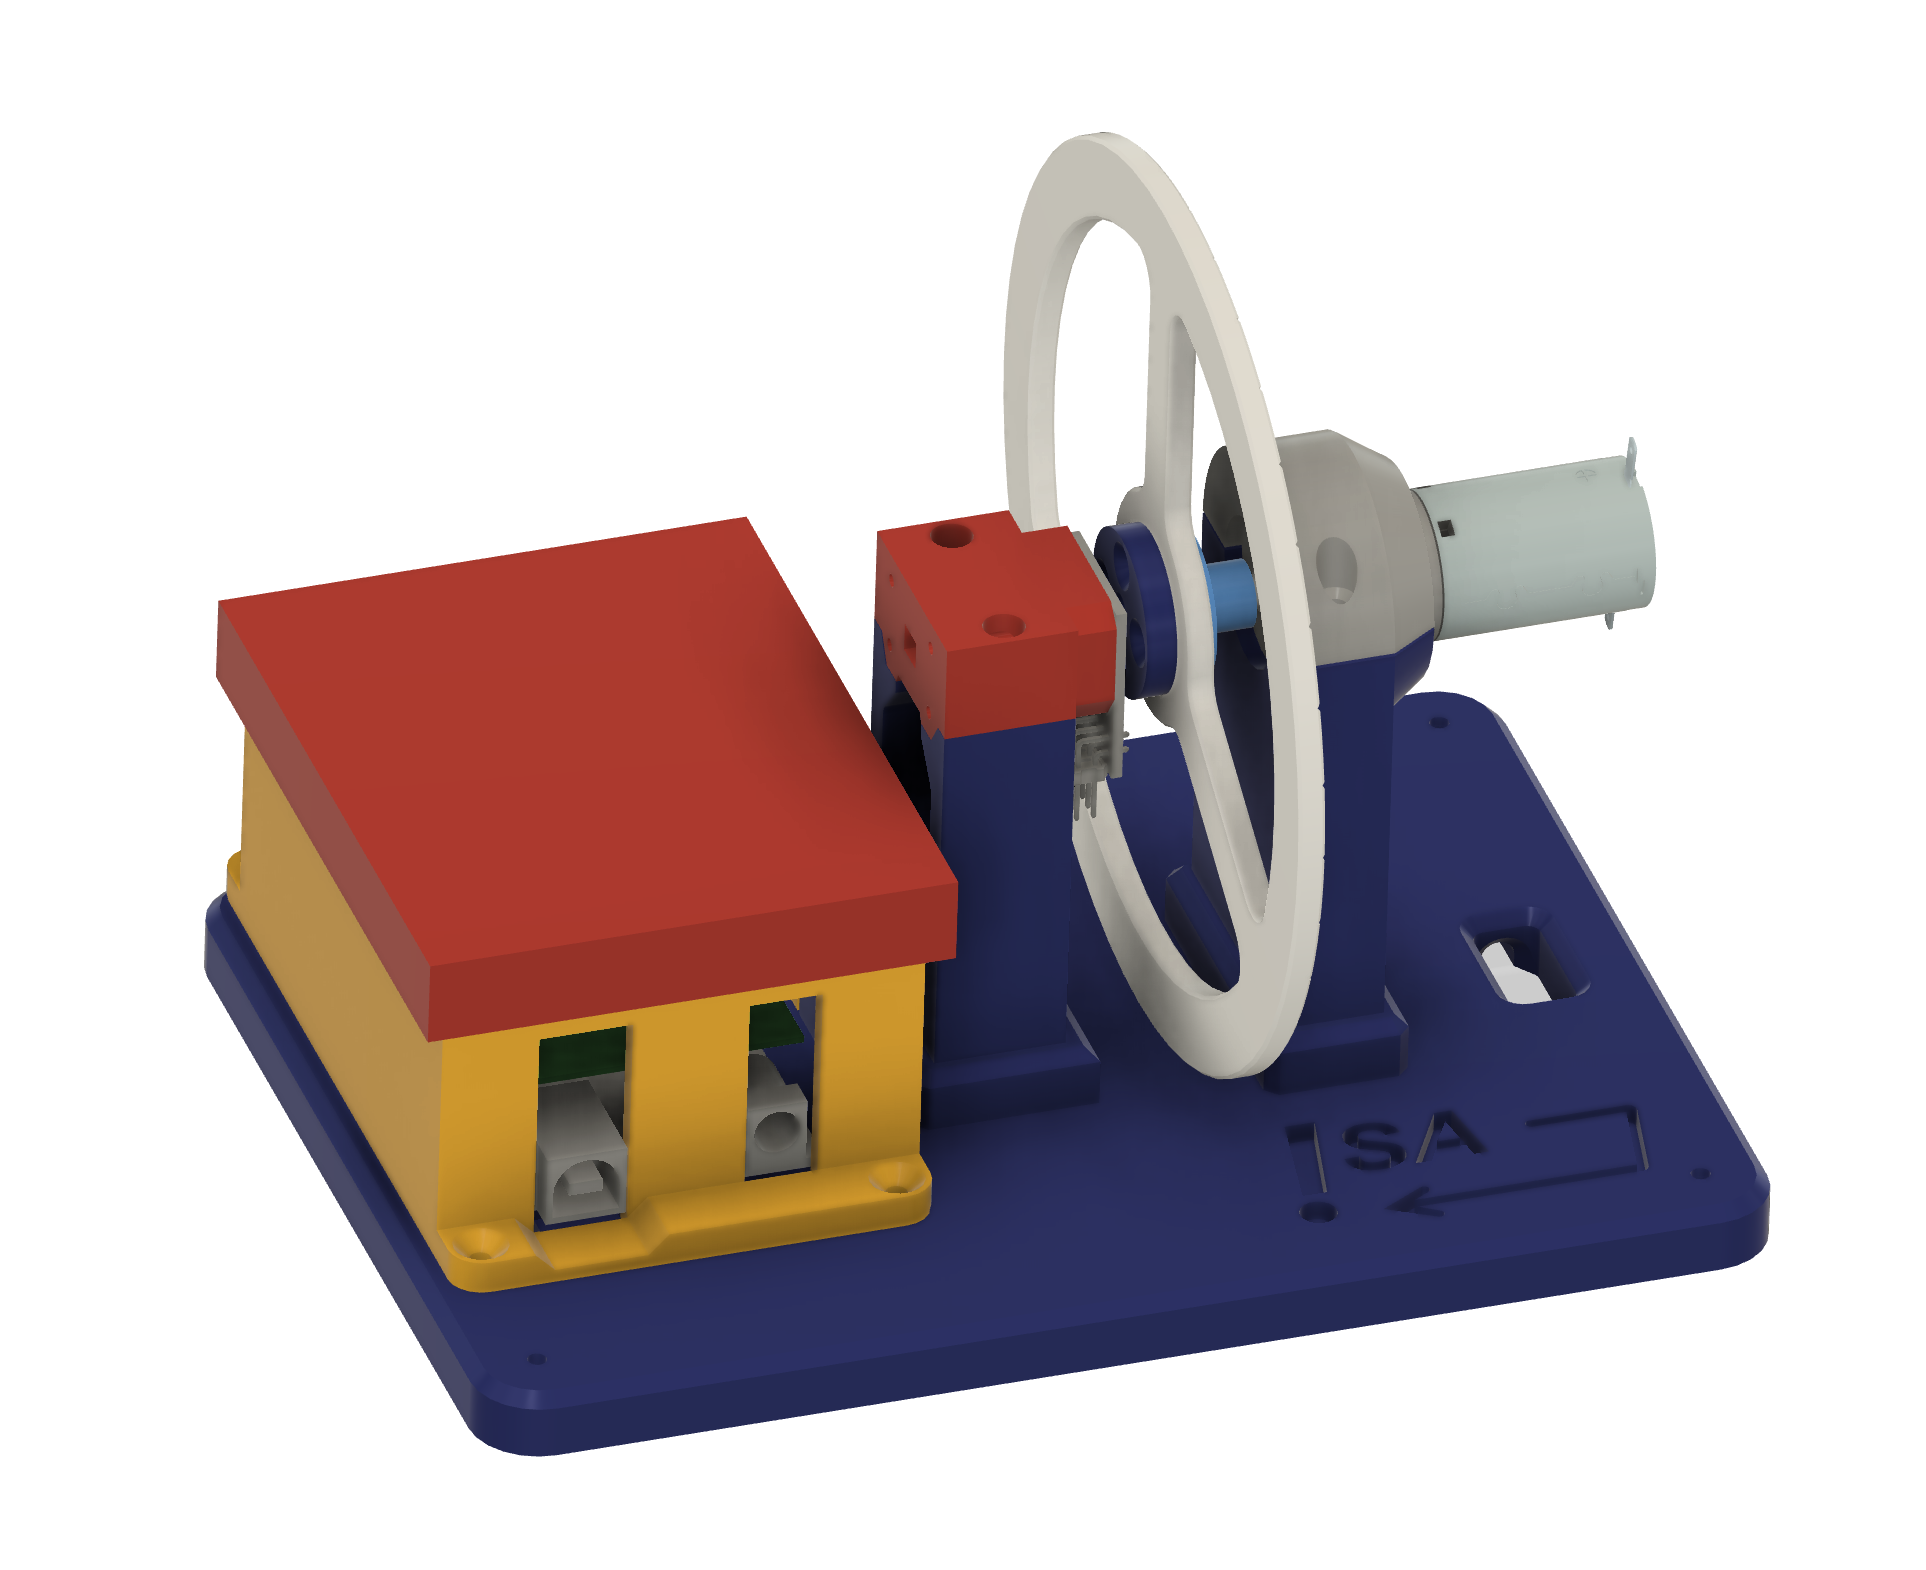
\includegraphics[width=\linewidth,height=2.3cm,keepaspectratio]{../images/equipo_render.png}
\end{minipage}\par
\smallskip\hrule\medskip

\textbf{When to use this guide.} Only to prepare a new Arduino, replace the board or update the firmware. If the rig already works, go straight to \texttt{user\_manual\_isa.pdf}. Uploaded firmware remains stored when Arduino is unplugged.

\section*{1. Prepare the computer}
You need Arduino IDE 2.x, an Arduino UNO, a USB data cable and a copy of the repository. MATLAB is not involved in uploading the firmware.

\textbf{Download the files first.} Open \href{https://github.com/DocMuerde/Motor-CC-Control-Lab}{github.com/DocMuerde/Motor-CC-Control-Lab}, click \textbf{Code > Download ZIP} and extract the ZIP into a folder on your computer.

\textbf{Alternative using Git.} If you have Git, open a terminal in the folder where you want to save the project and run:\par
{\small\ttfamily git clone https://github.com/DocMuerde/Motor-CC-Control-Lab.git}\par
In either case, locate the extracted or cloned folder: it contains \texttt{firmware/arduino/main/main.ino}. Do not open the file from inside the ZIP.

\textbf{Install the Arduino libraries}
\begin{enumerate}
\item Open Arduino IDE and its \textbf{Library Manager}.
\item Find and install \textbf{AS5047P} by Marginally Clever. This is the library used by \texttt{\#include <AS5047P.h>}.
\item Find and install \textbf{MsTimer2}. This is the library used by \texttt{\#include <MsTimer2.h>}. Built-in Arduino core libraries come with the board environment.
\end{enumerate}
These libraries are needed on the computer that compiles and uploads the firmware; they are not needed on every computer running the rig from MATLAB.

\clearpage
{\small\color{isa} Firmware installation · Arduino UNO}\par
\section*{2. Upload the program}
\begin{enumerate}
\item Leave external power disconnected and connect Arduino to the computer by USB. Keep the motor shaft clear. Close simulations and any program using the serial port.
\item In Arduino IDE, select \textbf{File > Open} and, inside the downloaded or cloned folder, open \texttt{firmware/arduino/main/main.ino}. Keep the folder name \texttt{main} and the file name \texttt{main.ino}.
\item Under \textbf{Tools > Board}, select \textbf{Arduino Uno} from \textbf{Arduino AVR Boards}; install that package through Boards Manager if it is missing.
\item Under \textbf{Tools > Port}, select the Arduino port. If unsure, unplug and reconnect USB to identify the port that appears.
\item Click \textbf{Verify} to compile. If a missing-library error appears, check the two libraries listed above.
\item Click \textbf{Upload} and wait for confirmation that the upload completed without errors.
\end{enumerate}

\section*{3. Check and switch to MATLAB}
For a basic check, you can open \textbf{Serial Monitor} at \textbf{115200 baud}. The firmware sends binary packets every 10 ms, so unreadable symbols are expected. If encoder initialization fails, the firmware prints an SPI connection error every 5 s. Serial activity alone does not verify the motor drive. Do not send text commands.

\textbf{Close Serial Monitor} to release the port. Follow the quick start guide: open the model for your MATLAB release, double-click \textbf{Motor CC}, select the port, click \textbf{OK}, then \textbf{Run}. Check position and velocity readings in the Scopes.

\textbf{Upload fails?} Check board and port selection, close Serial Monitor and MATLAB, and try another USB data cable. If measurements are missing, check the shield and encoder connections with the rig disconnected.

\textbf{Separate dependencies:} using the rig requires MATLAB with Simulink and \textbf{Instrument Control Toolbox} as the only additional toolbox. The Arduino libraries above are used only to install or update the firmware.
\end{document}
